\section{Actividades Encargadas} 

\subsection {¿Con qué comando(s) exportaría la imagen de Docker de Microsoft SQL Server a otra PC o servidor?}
\begin{itemize}
	\item El comando usado para exportar es el siguiente:
	
	\begin{center}
	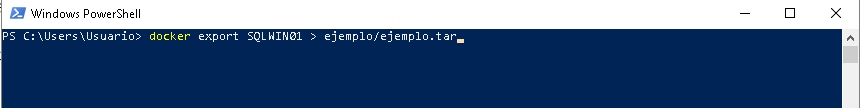
\includegraphics[width=17cm]{./Imagenes/Actividad1} 
	\end{center}

\item De tal modo que se genera un archivor .tar el cual se podra transportar a otra maquina (Windows o Linux).
	\begin{center}
	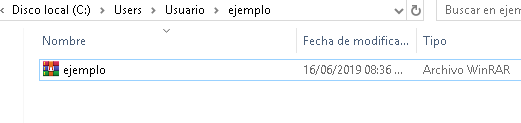
\includegraphics[width=15cm]{./Imagenes/Actividad2} 
	\end{center}
\end{itemize} 
\subsection {¿Con qué comando(s) podría generar dos volúmenes para un contenedor para distribuir en un volumen el Archivo
de Datos (.mdf) y en otro el Archivo Log (.ldf)?}
\begin{itemize}
\item Los comandos para generar dos volúmenes para un contenedor son los siguientes:
\begin{center}
	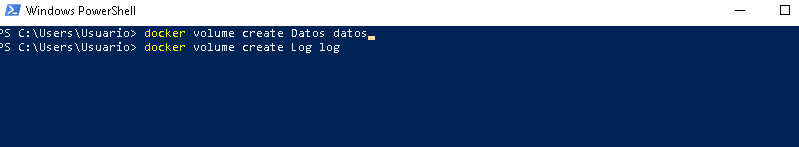
\includegraphics[width=15cm]{./Imagenes/Actividad3} 
	\end{center}
\end{itemize} 

\subsection {Genere un nuevo contenedor y cree la base de datos con las siguientes características.}
\begin{itemize}
\item El Script es:



\begin{center}
	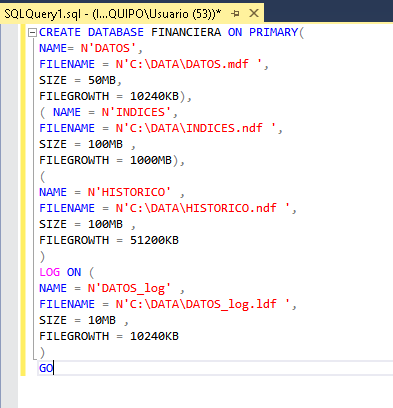
\includegraphics[width=10cm]{./Imagenes/Actividad4} 
	\end{center}

\end{itemize} 